\documentclass[11pt]{article}
\usepackage{graphicx} % This lets you include figures
\usepackage{hyperref} % This lets you make links to web locations
\usepackage[margin=0.5in]{geometry}
\usepackage[rightcaption]{sidecap}
\usepackage{subcaption}
\usepackage{wrapfig}
\usepackage{float}
\usepackage{imakeidx}
\usepackage{indentfirst}
\makeindex
%---------------------------Do Not Edit Anything Above This Line!!------------------------

% edit the line below, if needed, to change the directory name for your image files.
\graphicspath{ {./images/} }



\begin{document}

%---------------------------Edit Content in the Box to Create the Title Page--------------
\begin{titlepage}
   \begin{center}
       \vspace*{1cm}
	   \Huge
       \textbf{Complexity Analyzer}

       \vspace{0.5cm}
       \Large
       Project 3 \\
       10/27/2025 \\
   \end{center}

       \vspace{1.5cm}

\begin{table}[h!]
\centering
\begin{tabular}{|l|l|}
\hline
\textbf{Name} & \textbf{Email Address} \\ \hline
Aaron Downing         & aaron.downing652@topper.wku.edu         \\ \hline
Ryerson Brower         & ryerson.brower178@topper.wku.edu         \\ \hline
\end{tabular}
\end{table}

%Latex Table Generator    
%https://www.tablesgenerator.com/     
        
\vspace{4in}

\centering        
CS 396 \\
Fall 2024\\
Project Organization Documentation

\end{titlepage}
%---------------------------Edit Content in the Box to Create the Title Page--------------


% No text here.


%---------------------------Do Not Edit Anything In This Box!!------------------------
%Table of contents and list of figures will be autogenerated by this section.
\newpage
\setcounter{page}{1}%
\cleardoublepage
\pagenumbering{gobble}
\tableofcontents
\cleardoublepage
\pagenumbering{arabic}
\clearpage
\newpage
\setcounter{page}{1}%
\cleardoublepage
\pagenumbering{gobble}
\listoffigures
\cleardoublepage
\pagenumbering{arabic}
\newpage
%---------------------------Do Not Edit Anything In This Box!!------------------------

% No text here.


%---------------------------Project Team's Organizational Approach------------------------------
\section{Project Team's Organizational Approach} %\section{} is used to create major section headers
%How/where did the group meet?  How often did you meet as an entire team? 
	
For this project we tried to meet every so often at the commons to work on coding the Complexity Analyzer. When we would meet at the commons we tried to be there for about an hour or 2. With these meeting we finished the coding which was the hardest part. We also talked a lot over text and call to work on the documents. Because we didn’t think to much of having to meet to finish the documents.

%---------------------------End Project Team's Organizational Approach------------------------------


% No text here.


%---------------------------Schedule Organization---------------------------------------------------
\section{Schedule Organization}
%Gantt charts cover the tasks/time commitments and estimations for the entire project.  We will have four iterations of the Gantt Chart, with iteration focusing on a specific sprint.

\subsection{Gantt Chart:}
%100 words to describe the focus for this sprint.
%Identify the location for the Gantt Chart.  Should be clearly labeled in the project directory.

\begin{figure}[h]
   \centering
    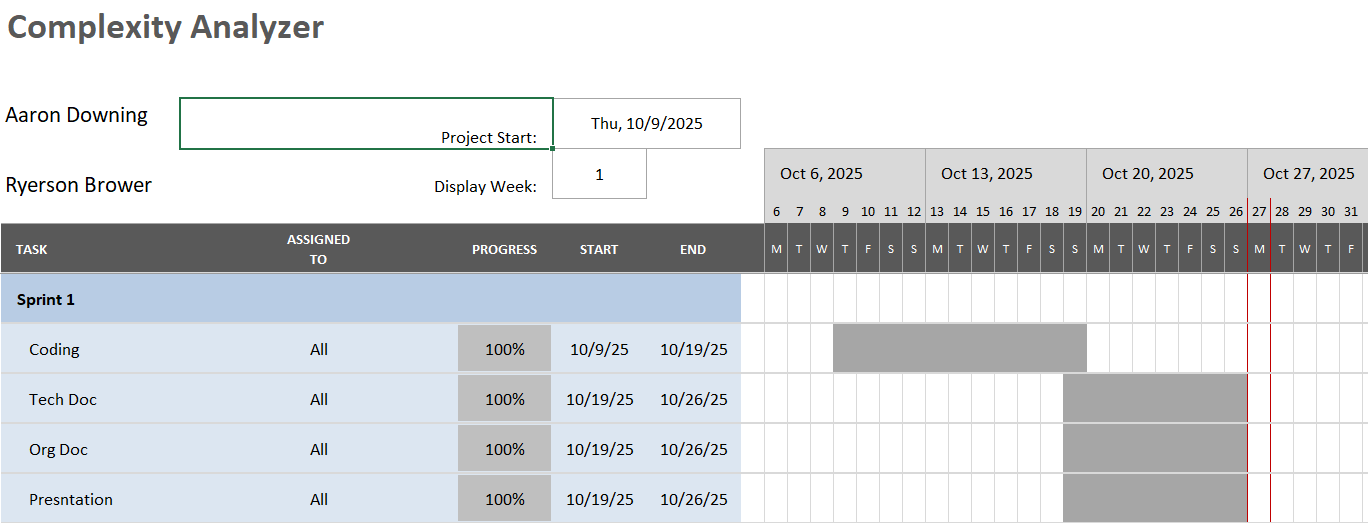
\includegraphics[scale=0.7]{Gannt Chart.png} 
    \caption{Our Gannt chart for project 3.}
        \label{fig16}
\end{figure}


%---------------------------End Schedule Organization---------------------------------------------------


% No text here.


%---------------------------Progress Visibility---------------------------------------------------
\section{Progress Visibility}
%Explain how each member of the group is progressing with assigned tasks and how that progress is shared with the group.  Examples:  how does the group assign tasks?  How to group members know tasks assigned to them?  How do group members communicate when assigned tasks are complete, need assistance, or waiting on other tasks to be completed first?

Through this project we kept as much contact as we could to keep up with every change and different tasks that were completed. We didn’t really assign any specific tasks. This is because for the most part we mainly worked together on it. Our meetings would consist of coding the Complexity Analyzer. After that we split up the sections of
the documents and assigned them for faster completion of the docs and presentation. To help with version control we used git hub so that it was pretty easy to keep each other up to date on our codes and the updated documents. We also used git actions to help with deployment. 

%---------------------------End Progress Visibility---------------------------------------------------


% No text here.


%---------------------------Risk Management--------------------------------------------------------------
\section{Risk Management}
%Use this section to describe the team's approach to risk management.
For our risk management we as said above we worked mostly together on the coding so that whenever we ran into a error we could work on it together and fix it there. For the most part this worked wonders we didn’t have to many problems along the way. The weirdest thing to get set up was GIT actions we never used it before so it was a bit weird to us.


%---------------------------Risk Management--------------------------------------------------------------








%example links:  uncomment to show usage.
%\url{https://www.youtube.com}
%\href{https://www.wku.edu/}{WKU Homepage}
%\footnote{You can put the link in a footnote like this.}

% Anything to the right of a percent sign will be ignored by LaTeX.
% You can use this to put notes to yourself.  



\end{document}
